\subsection{Bernoulli}
\paragraph{Purpose}
To estimate the outcome of an experience providing binary outcomes.
\paragraph{Theory}
\subparagraph{Parameters}
$p$ such that $\prob{X=1} = p$.
\subsection{Binomial}
\subparagraph{Purpose}
It estimates the \uB{number of successes in a sequence of $n$ independent experiments} having binary
outcomes.
\subparagraph{Parameters}
\begin{itemize}
    \item $n$: number of independent experiments
    \item $p$: probability of success, $\prob{X=1} = p$
    \item $f(k, n, p) = \prob{X=k} = \binom{n}{k}p^{k}(1-p)^{n-k}$ the probability mass function
        giving the probability to get exactly $k$ successes over $n$ independent experiments.
\end{itemize}

\begin{figure}[H]
    \begin{center}
        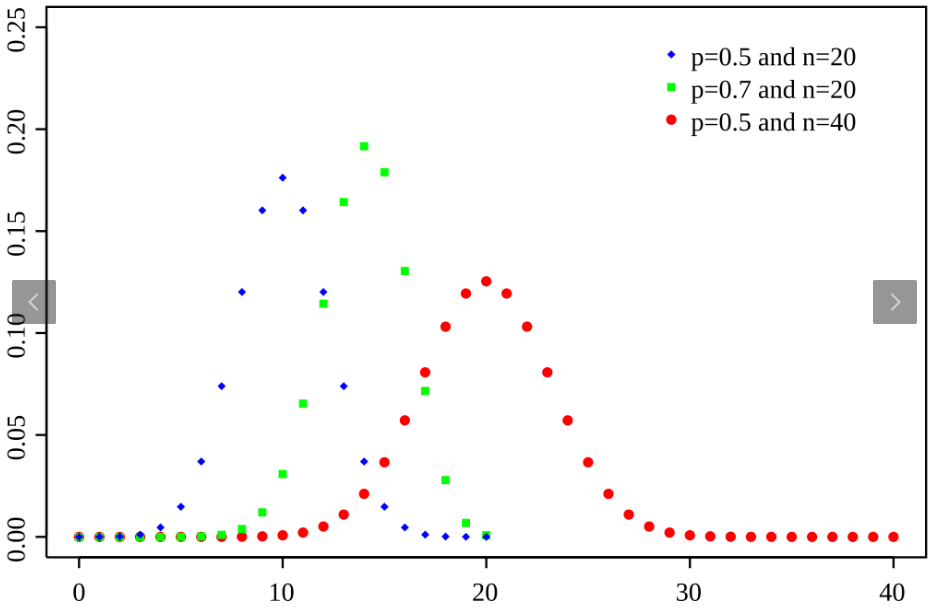
\includegraphics[width=.5\textwidth]{./chapters/2_statistics/02_common_probability_distributions/images/01_binomial_pmf.png}
    \end{center}
    \caption{Binomial probability mass function}
    \label{fig:01_binomial_pmf}
\end{figure}

\subparagraph{Approximation}
\begin{itemize}
    \item \emph{Normal distribution}: when $n$ becomes large enough the \emph{skew} gets lower and
        a reasonable approximation of $\mathcal{B}(n, p) \sim \mathcal{N}\left(np, np(1-p)\right)$
    \item \emph{Poisson distribution}: when $n\rightarrow\infty \wedge np\rightarrow C$ ($n$ should 
        be sufficiently large and $p$ sufficiently small)
        $\mathcal{B}(n, p) \sim \mathcal{P}(np)$ kn
    \item \emph{Beta distribution}: when $\alpha=k+1 \wedge \beta=n-k+1$ we have 
        $Beta(p,\alpha,\beta) = (n+1)Binomial(k, n, p)$
\end{itemize}

\subsection{Beta-Binomial}
\paragraph{Purpose}

\subsection{Degenerate}
\subsection{Uniform}
\subsection{Hypergeometric}
\subsection{Negative Hypergeometric}
\subsection{Poisson Binomial}
\subsection{Fisher's noncentral hypergeometric}
\subsection{Benford's law}
\subsection{Zipf's law}
\subsection{Zipf-Mandelbrot law}

